\chapter{Preâmbulo matemático}
\textsl{{\sffamily(Versão: \today)}}

\section{Produto escalar e produto vetorial de vetores}
\subsection*{Produto escalar ou interno}
Dados dois vetores, define-se o seu \emph{produto escalar} (ou \emph{produto
interno}) como o escalar que se obtém multiplicando os módulos dos dois vetores
e o cosseno do ângulo entre eles. Assim, se $\vec a$ e $\vec b$ forem os dois
vetores e $\theta$ for o ângulo que definem, o produto escalar
é\footnote{Nestes apontamentos usa-se uma convenção tipográfica usual em física,
  em que se representa o módulo de um vetor $\vec a$ por $a$: a mesma letra, mas
sem a setinha por cima.}
\begin{equation}
  \vec a\cdot\vec b= ab\cos\theta.
\end{equation}
É imediato verificar que o produto escalar de dois vetores pode ser positivo (se
o ângulo entre eles for menor que 90\deg), negativo (se for maior que 90\deg) ou
nulo (se os dois vetores forem perpendiculares). Verifica-se também
que este produto é comutativo, isto é, $\vec a\cdot\vec b=\vec b\cdot\vec a$.

Sejam respetivamente $(a_x,\,a_y,\,a_z)$ e $(b_x,\,b_y,\,b_z)$ as componentes
dos vetores $\vec a$ e $\vec b$ relativamente a alguma base ortonormada
pré-escolhida, formada por versores (vetores com norma 1) $\he_x$, $\he_y$ e
$\he_z$. Isto quer dizer que estes dois vetores se podem escrever como as
combinações lineares dos vetores da base seguintes
\begin{align*}
  \vec a&=a_x\he_x+a_y\he_y+a_z\he_z&
  \vec b&=b_x\he_x+b_y\he_y+b_z\he_z.
\end{align*}
O produto escalar destes dois vetores pode então desenvolver-se como
\begin{align*}
  \vec a\cdot\vec b&=
  (a_x\he_x+a_y\he_y+a_z\he_z) \cdot (b_x\he_x+b_y\he_y+b_z\he_z)\\
  &=a_xb_x(\he_x\cdot\he_x)+ a_xb_y(\he_x\cdot\he_y)+ a_xb_z(\he_x\cdot\he_z)\\
  &+a_yb_x(\he_y\cdot\he_x)+ a_yb_y(\he_y\cdot\he_y)+ a_yb_z(\he_y\cdot\he_z)\\
  &+a_zb_x(\he_z\cdot\he_x)+ a_zb_y(\he_z\cdot\he_y)+ a_zb_z(\he_z\cdot\he_z)
\end{align*}
Mas os produtos escalares de versores da base diferentes são nulos (porque eles
são todos perpendicuares entre si) e os produtos escalares de um qualquer versor
da base consigo próprio é 1 (porque o módulo dos versores é 1 e o cosseno do
ângulo [nulo] que um vetor faz consigo próprio também é 1), isto é,
\begin{align*}
  \he_x\cdot\he_x=\he_y\cdot\he_y=\he_z\cdot\he_z=1\\
  \he_x\cdot\he_y=\he_y\cdot\he_z=\he_z\cdot\he_x=0.
\end{align*}
Substituindo em cima, obtemos uma forma alternativa para o produto escalar de
dois vetores:
\begin{equation}\label{eq:dprod}
  \vec a\cdot\vec b=a_xb_x+a_yb_y+a_zb_z.
\end{equation}

\subsection*{Produto vetorial ou externo}
Define-se também o \emph{produto vetorial} ou \emph{produto externo} de vetores.
Como o próprio nome indica, o produto vetorial de dois vetores é ainda um
vetor.
A norma do produto escalar de dois vetores é o produto
das suas normas e do seno do ângulo entre eles:
\begin{equation}
  \|\vec a\times\vec b\|=ab\sin\theta;
\end{equation}
a sua direção é a perpendicular ao plano definido pelos dois vetores que se
multiplicam e o sentido é o definido pela regra da mão direita\footnote{%
  \parbox[t]{0.8\textwidth}{Há várias formas de enunciar esta regra, pode
    encontrá-las todas rapidamente numa pesquisa na web (experimente usar
    ``cross product right hand rule'' como expressão de busca). Escolha a que
    preferir. Eu gosto desta: oriente o indicador da mão direita como o primeiro
    vetor no produto e o médio da mesma mão como o segundo; o polegar indica
  então o sentido do produto vetorial (veja a figura ao lado, retirada da
  Wikipedia)}\hfill
  \parbox[t]{1.8cm}{%
    \raisebox{-0.8\height}{%
      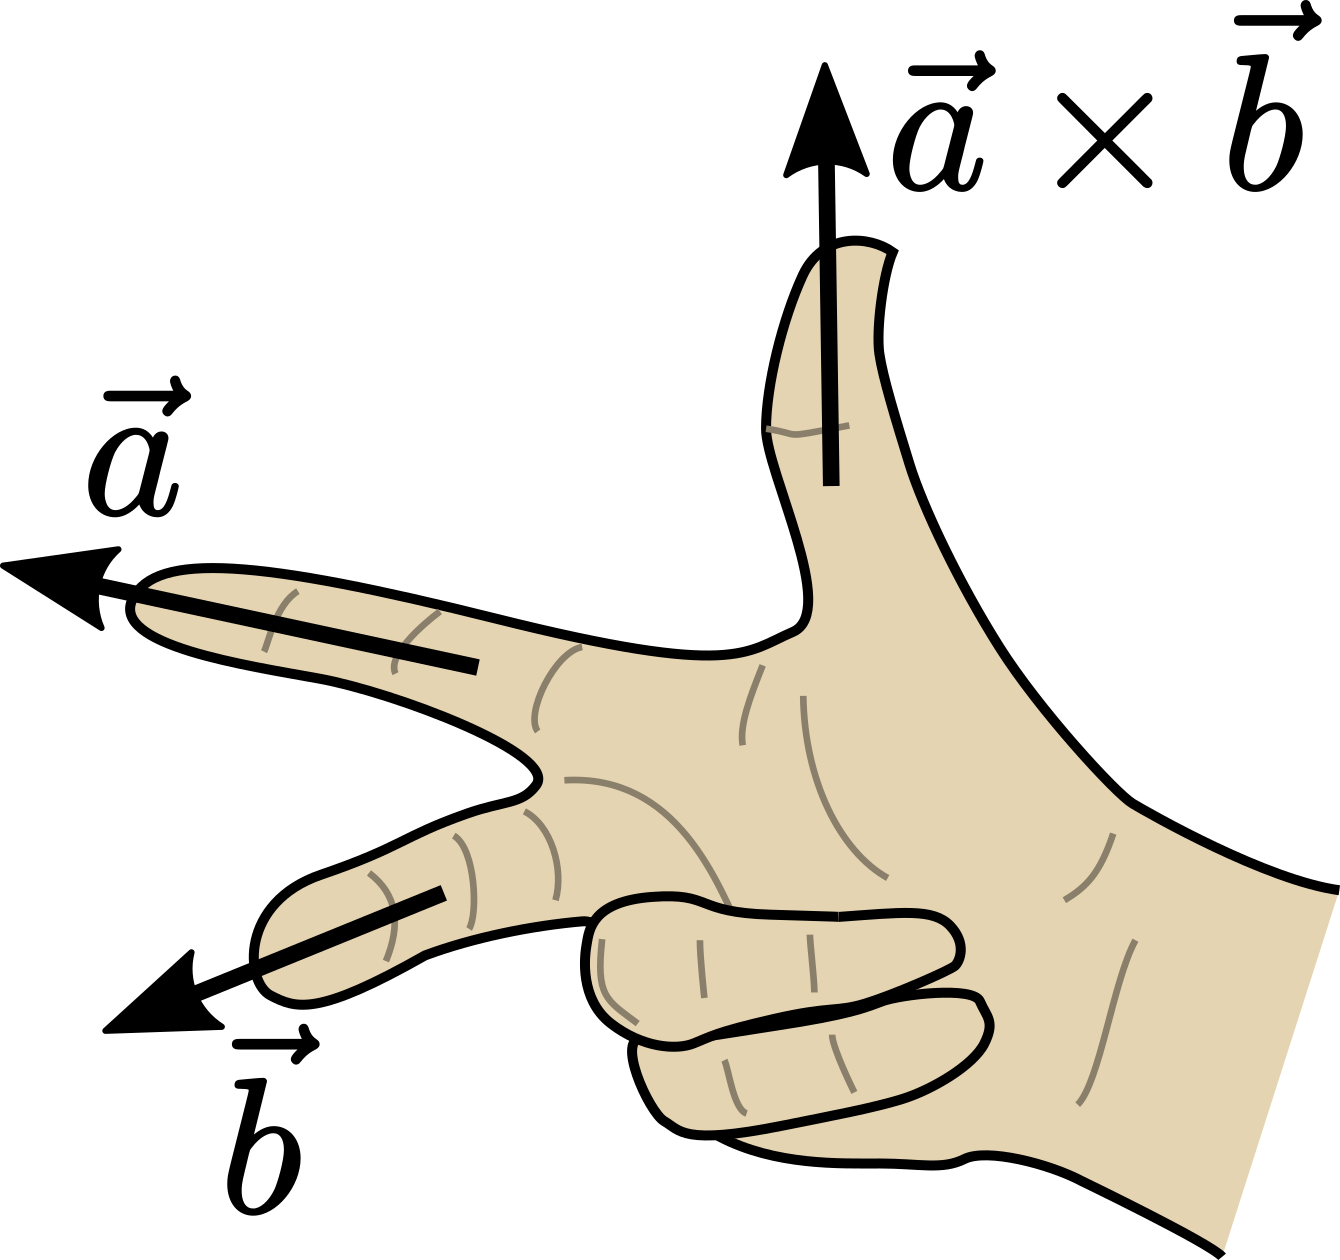
\includegraphics[width=1.7cm]{figs/f10-010.png}
    }
  }
}.
O produto vetorial assim definido é \emph{anticomutativo}, isto é, o sinal do
resultado é trocado se trocarmos a ordem dos fatores: $\vec a\times\vec b=-\vec
b\times\vec a$. Constata-se também que
\begin{align}
  \he_x\times\he_y&=\he_z&
  \he_y\times\he_z&=\he_x&
  \he_z\times\he_x&=\he_y.
\end{align}
Munidos destas igualdades (e das que resultam trocando a ordem dos fatores nos
seus lados esquerdos) obtemos uma expressão para o cálculo do vetor produto
vetorial em termos das componentes dos dois vetores multipicados externamente.
Sejam, como há pouco, $a_x,\,a_y,\,a_z$ e $b_x,\,b_y,\,b_z$ as componentes de
dois vetores $\vec a $ e $\vec b$ relativamente a uma base ortonormada formada
por vetores unitarios $\he_x$ $\he_y$, $\he_z$. Então,
\begin{equation*}
  \vec a = a_x\he_x+a_y\he_y+a_z\he_z\rule{2cm}{0mm}
  \vec b = b_x\he_x+b_y\he_y+b_z\he_z,
\end{equation*}
e, assim,
\begin{align*}
  \vec a \times \vec b &=
  (a_x\he_x+a_y\he_y+a_z\he_z)\times
  (b_x\he_x+b_y\he_y+b_z\he_z)\\
  &=
  (a_yb_z-a_zb_y)\he_x+(a_zb_x-a_xb_z)\he_y+(a_xb_y-a_yb_x)\he_z.
\end{align*}
Esta expressão para o produto vetorial de dois vetores em termos das componentes
dos vetores multiplicados é fácil de memorizar notando que pode também ser vista
como o determinante da matriz simbólica (verifique):
\begin{equation}
  \vec a\times\vec b =\det
  \begin{bmatrix}
    \he_x&\he_y&\he_z\\
    a_x&a_y&a_z\\
    b_x&b_y&b_z
  \end{bmatrix}.
\end{equation}

O produto vetorial não é comutativo (é anticomutativo, como vimos) e também não
é associativo. O produto vetorial de três vetores satisfaz as igualdades
\begin{equation}\label{eq:tcp}
\begin{split}
\vec a\times(\vec b\times\vec c)&=\vec b(\vec a\cdot\vec c)-(\vec a\cdot\vec
b)\vec c\\
(\vec a\times\vec b)\times\vec c&=\vec b(\vec a\cdot\vec c)-\vec a(\vec
b\cdot\vec c)
\end{split}
\end{equation}

\subsection*{Áreas de paralelogramos e volumes de paralelipípedos}
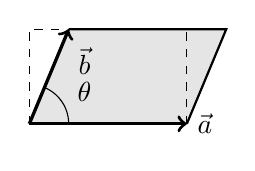
\begin{tikzpicture}[baseline=(current bounding box.north)]
%\small
\coordinate(O) at (0,0);
\coordinate(a) at (2,0);
\coordinate(b) at (0.5,1.2);
\coordinate(ab) at (2.5,1.2);
\fill [gray!20] (O) -- (a) -- (ab) -- (b) --cycle;
\draw [very thick, ->] (O) --(a) node[right]{$\vec a$};
\draw [very thick, ->] (O) --(b) node[shift={(2mm,-4mm)}]{$\vec b$};
\draw [thick] (a) -- (ab) -- (b);
\draw [dashed] (O) -- (O|-b) --(b);
\draw [dashed] (a) -- (a|-b);
\begin{scope}
\clip (b)--(O) --(a);
\draw (O) circle (0.5cm) node[shift={(7mm,4mm)}] {$\theta$};
\end{scope}
\end{tikzpicture}
\hfill
\begin{minipage}[t]{0.8\textwidth}
Consideremos a área do paralelogramo formado por dois vetores $\vec a$ e $\vec
b$ (ver a figura ao lado). Seja $\theta$ o ângulo entre os dois vetores.
Claramente, aquela área é igual à do retângulo com base $a=\|\vec a\|$ e altura
$b\sin\theta$, igual à do paralelogramo inicial. A área considerada é pois
\end{minipage}
\begin{equation}
A=ab\sin\theta=\|\vec a\times\vec b\|.
\end{equation}

Consideremos agora um terceiro vetor $\vec c$, não coplanar com $\vec a$ e $\vec
b$. Seja $\phi$ o ângulo entre $\vec c$ e a normal ao plano definido pelos
vetores $\vec a$ e $\vec b$. Com um argumento semelhante ao que acabámos de
usar para calcular a área de um paralelogramo, prova-se que o volume deste
paralelipípedo é
\begin{equation}
V=b\cos\phi A = c \|\vec a\times\vec b\| \cos\phi=
\left|\vec c\cdot\vec a\times\vec b\right|.
\end{equation}

\section{Sistemas de coordenadas e bases de vetores}
Um sistema de coordenadas é uma forma de especificar numericamente a posição de
cada ponto no espaço. Porque o espaço em que nos movemos é tridimensional (as
porções do espaço podem ter largura, comprimento e altura), são em geral necessários
três números (três coordenadas) para definir completamente a posição de cada
ponto. Em certas situações, a posição dos objetos considerados pode estar
constrangida de algum modo e, por isso, bastarem dois (como a latitude e a
longitude de um ponto na superfície da Terra) ou apenas um (o \emph{quilómetro}
onde se dá um acidente numa autoestrada) para a especificar; nestes
casos, o espaço considerado é apenas bi- ou unidimensional.

O sistema de coordenadas usado em cada problema é definido como for considerado
mais conveniente. Qualquer problema pode ser analisado com qualquer sistema de
coordenadas, mas a complexidade algébrica da análise pode ser muito diferente
usando diferentes sistemas.

Os sistemas mais frequentemente usados em física (mas de modo algum os únicos)
são os seguintes (veja a Figura~\ref{fig:10-015}):
\begin{itemize}
\item\textbf{coordenadas cartesianas $(x,\,y,\,z)$}\\
    O sistema de coordenadas mais familiar é o das coordenadas cartesianas.
    Escolhido um ponto (a origem) e três direções perpendiculares entre si (os
    \emph{eixos coordenados} das coordenadas $x$, $y$ e $z$, indicamos a posição
    de um ponto dado pelas distâncias que o separam de cada um dos planos
    definidos por cada par de eixos coordenados, eventualmente afetadas de um
    sinal para indicar de que lado de cada plano se encontra o ponto.
\item\textbf{coordenadas polares esféricas $(r,\,\theta,\,\phi)$}\\
    Outro sistema muito usual é o das coordenadas polares esféricas. Escolhida a
    origem, uma direção que a contém (o eixo \emph{polar} e um plano que contem
    o eixo (plano de referência azimutal), a posição
    de um ponto é indicada pela sua distância à origem $r$ , pelo ângulo (chamado
    \emph{ângulo polar}) que a linha que o une à origem faz com o eixo polar
    $\theta$ e pelo ângulo (\emph{ângulo azimutal}) que essa linha faz com o
    plano de referência azimutal $\phi$.
\item\textbf{coordenadas polares cilíndricas $(\rho,\,z,\,\phi)$}\\
    De certa maneira, o sistema de coordenadas polares cilíndricas é um misto
    das coordenadas cartesianas e das coordenadas polares esféricas. Com nas
    coordenadas esféricas, escolhe-se uma origem, um eixo polar e um plano de
    referência azimutal; a partir daí, usa-se a distância $\rho$ do ponto ao
    eixo polar (atenção: é a distância ao eixo, não a distância à origem), a
    a distância $z$ do ponto ao plano perpendicular a esse eixo que contém a
    origem (corresponde à coordenada cartesiana $z$ se tomarmos o eixo polar
    como eixo dos $z$) e o ângulo azimutal para especificar a sua posição.
\end{itemize}
\begin{figure}[htb]
{\centering
\tdplotsetmaincoords{65}{120}
%
\pgfmathsetmacro{\rvec}{0.9}
\pgfmathsetmacro{\thetavec}{30}
\pgfmathsetmacro{\phivec}{50}
%
\begin{tikzpicture}[scale=3,tdplot_main_coords]
    % Cartesian
    \begin{scope}[xshift=-1.5cm]
        \coordinate (O) at (0,0,0);
        \draw[->] (O) -- (0.5,0,0);  %x
        \draw[->] (O) -- (0,0.5,0);  %y
        \draw[->] (O) -- (0,0,0.88); %z

        \tdplotsetcoord{P}{\rvec}{\thetavec}{\phivec}
        \draw[-stealth] (O) -- (P) node[above right] {$P$};
        \draw [thin, dashed] (O) -- (Pxy);
        \draw [thin, dashed] (P) -- (Pxy);
        \draw [thin, dashed] (P) -- (Pz) node[left]{$z$};
        \draw [thin, dashed] (Px) node [above] {$x$} --(Pxy)--(Py) node[above]
        {$y$};
    \end{scope}
    % Polar Spherical
    \begin{scope}
        \coordinate (O) at (0,0,0);
        \draw[->] (O) -- (0.5,0,0);  %x
        \draw[->] (O) -- (0,0.5,0);  %y
        \draw[->] (O) -- (0,0,0.88); %z

        \tdplotsetcoord{P}{\rvec}{\thetavec}{\phivec}
        \draw[-stealth] (O) -- (P) node[above right] {$P$}
            node [pos=0.7, shift={(0.0,0.05,-0.25)}] {$r$};
        \draw [thin, dashed] (O) -- (Pxy);
        \draw [thin, dashed] (P) -- (Pxy);
        \draw [thin, dashed] (P) -- (Pz);
        %\draw [thin, dashed] (Px) --(Pxy)--(Py);

        \tdplotdrawarc[thin]{(O)}{0.25}{0}{\phivec}{anchor=north}{$\phi$}
        \tdplotsetthetaplanecoords{\phivec}
        \tdplotdrawarc[tdplot_rotated_coords,thin]{(0,0,0)}{0.4}{0}%
            {\thetavec}{anchor=south,xshift=1.5}{$\theta$}
    \end{scope}
    % Polar Cilyndrical
    \begin{scope}[xshift=1.5cm]
        \coordinate (O) at (0,0,0);
        \draw[->] (O) -- (0.5,0,0);  %x
        \draw[->] (O) -- (0,0.5,0);  %y
        \draw[->] (O) -- (0,0,0.88); %z

        \tdplotsetcoord{P}{\rvec}{\thetavec}{\phivec}
        \draw[-stealth] (O) -- (P) node[above right] {$P$};
        \draw [thin, dashed] (O) -- (Pxy);
        \draw [thin, dashed] (P) -- (Pxy);
        \draw [thin, dashed] (P) -- (Pz) node[left]{$z$} node
        [midway,shift={(2pt,5pt)}]{$\rho$};
       % \draw [thin, dashed] (Px) --(Pxy)--(Py);

        \tdplotdrawarc[thin]{(O)}{0.25}{0}{\phivec}{anchor=north}{$\phi$}
        \tdplotsetthetaplanecoords{\phivec}
    \end{scope}
\end{tikzpicture}\par
}
\caption{Coordenadas cartesianas $(x,\,y,\,z)$ (à esquerda), coordenadas polares
esféricas $(r,\,\theta,\,\phi)$ (ao centro) e coordenadas polares cilíndricas
$(\rho,\,z,\,\phi)$ (à direita).\label{fig:10-015}}
\end{figure}

Escolhendo para eixo polar o eixo da coordenada cartesiana $z$ e o plano de
referência polar coincidente com o plano $zx$, as relações entre as coordenadas
cartesianas e as coordenadas polares (esféricas e cilíndricas) é 
\begin{align*}
x&=r\sin\theta\cos\phi&
    r&=\sqrt{x^2+y^2+z^2}\hspace{2.0cm}&
    x&=\rho\cos\phi&
    \rho&=\sqrt{x^2+y2}\\
y&=r\sin\theta\sin\phi&
    \theta&=\arccos\frac{z}{r}&
    y&=\rho\sin\phi&
    \phi&=\arctan\frac{y}{x}
    \\
    z&=r\cos\theta&
    \phi&=\arctan\frac{y}{x}&
    z&=z&
\end{align*}

Quando lidamos com variáveis vetoriais, é conveniente dispormos de \emph{bases}
de vetores, que usamos para as descrever. Por exemplo, o vetor aceleração da
gravidade perto da superfície da Terra tem direção vertical, é dirigido para
baixo e o seu módulo é 9,8\,m/s$^2$. Escolhendo uma base formada por dois
versores (vetores com norma unitária) horizontais $\he_x$ e $\he_y$ e um
terceiro vetor $\he_z$ vertical, orientado para cima, podemos resumir esta
descrição na expressão $\smash{\vec g=-9,8\,\text{m/s}^2}\,\he_z$ ou
$\smash{\vec g=(0,\,0,\,-9,8\,\text{m/s}^2)}$, usando outra notação habitual.
Qualquer destas notações só fica definida depois de estar escolhida a base
usada. 

Este problema da escolha da base é independente do da escolha do sistema de
coordenadas. Ainda assim, é usual escolherem-se os vetores que formam a base
vetorial paralelos, em cada ponto, aos eixos coordenados\footnote{Isto é, às
direções em que apenas uma das coordenadas varia.} nesse ponto, caso em
que chamamos à base assim definida base do sistema de coordenadas usado.
Assim, concretizando para o sistema de coordenadas cartesiano, mais familiar,
escolhemos o versor $\he_x$ da base das coordenadas cartesianas orientado na
direção em que a coordenada $x$ aumenta, ficando as restantes ($y$ e $z$)
constantes, e repetindo a lógica para os restantes vetores $\he_y$ e $\he_z$. Do
mesmo modo, o versor $\he_r$ da base das coordenadas esféricas tem, em cada
ponto, a direção em que a coordenada $r$ aumenta sem variarem as coordenadas
$\theta$ ou $\phi$. Tem pois a direção radial. A Figura~\ref{fig:10-016} ilustra
as orientações dos vetores das bases dos três sistemas de coordenadas referidos.
\begin{figure}[htb]
{\centering
\tdplotsetmaincoords{65}{120}
%
\pgfmathsetmacro{\rvec}{0.9}
\pgfmathsetmacro{\thetavec}{30}
\pgfmathsetmacro{\phivec}{50}
%
\begin{tikzpicture}[scale=3,tdplot_main_coords]
    % Cartesian
    \begin{scope}[xshift=-1.5cm]
        \coordinate (O) at (0,0,0);
        \draw[->] (O) -- (0.5,0,0);  %x
        \draw[->] (O) -- (0,0.5,0);  %y
        \draw[->] (O) -- (0,0,0.88); %z

        \tdplotsetcoord{P}{\rvec}{\thetavec}{\phivec}
        \draw[-stealth] (O) -- (P);
        \draw [thin, dashed] (O) -- (Pxy);
        \draw [thin, dashed] (P) -- (Pxy);
        \draw [thin, dashed] (P) -- (Pz) node[left]{$z$};
        \draw [thin, dashed] (Px) node [above] {$x$} --(Pxy)--(Py) node[above]
        {$y$};
        \draw [thick,->] (P) -- +(0,0,0.2) node[above]{$\hat e_z$};
        \draw [thick,->] (P) -- +(0,0.2,0) node[right]{$\hat e_y$};
        \draw [thick,->] (P) -- +(0.28,0,0) node[left]{$\hat e_x$};
    \end{scope}
    % Polar Spherical
    \begin{scope}
        \coordinate (O) at (0,0,0);
        \draw[->] (O) -- (0.5,0,0);  %x
        \draw[->] (O) -- (0,0.5,0);  %y
        \draw[->] (O) -- (0,0,0.88); %z

        \tdplotsetcoord{P}{\rvec}{\thetavec}{\phivec}
        \draw[-stealth] (O) -- (P)
            node [pos=0.7, shift={(0.0,0.05,-0.25)}] {$r$};
        \draw [thin, dashed] (O) -- (Pxy);
        \draw [thin, dashed] (P) -- (Pxy);
        \draw [thin, dashed] (P) -- (Pz);
        %\draw [thin, dashed] (Px) --(Pxy)--(Py);

        \tdplotdrawarc[thin]{(O)}{0.25}{0}{\phivec}{anchor=north}{$\phi$}
        \tdplotsetthetaplanecoords{\phivec}
        \tdplotdrawarc[tdplot_rotated_coords,thin]{(0,0,0)}{0.4}{0}%
            {\thetavec}{anchor=south,xshift=1.5}{$\theta$}
        \tdplotsetrotatedcoords{\phivec}{\thetavec}{0}
        \tdplotsetrotatedcoordsorigin{(P)}
        \draw[thick,tdplot_rotated_coords,->] (0,0,0)
            -- (.15,0,0) node[right]{$\hat e_\theta$};
        \draw [thick,tdplot_rotated_coords,->] (0,0,0) -- (0,0.14,0)
            node[right]{$\hat e_\phi$};
        \draw [thick,tdplot_rotated_coords,->] (0,0,0) -- (0,0,0.25)
            node[above]{$\hat e_r$};
    \end{scope}
    % Polar Cilyndrical
    \begin{scope}[xshift=1.5cm]
        \coordinate (O) at (0,0,0);
        \draw[->] (O) -- (0.5,0,0);  %x
        \draw[->] (O) -- (0,0.5,0);  %y
        \draw[->] (O) -- (0,0,0.88); %z

        \tdplotsetcoord{P}{\rvec}{\thetavec}{\phivec}
        \draw[-stealth] (O) -- (P);
        \draw [thin, dashed] (O) -- (Pxy);
        \draw [thin, dashed] (P) -- (Pxy);
        \draw [thin, dashed] (P) -- (Pz) node[left]{$z$} node
            [midway,shift={(-1pt,-6pt)}]{$\rho$};

        \draw [thick,->] (P) --+(0,0,0.17) node[above]{$\hat e_z$};
        \draw [thick,->] (P) -- ($ (P)!-0.15cm!(Pz) $) node [right]{$\hat
        e_\rho$};
        \tdplotdrawarc[thin]{(O)}{0.25}{0}{\phivec}{anchor=north}{$\phi$}
        \tdplotsetthetaplanecoords{\phivec}

        \tdplotsetrotatedcoords{\phivec}{\thetavec}{0}
        \tdplotsetrotatedcoordsorigin{(P)}
        \draw [thick,tdplot_rotated_coords,->] (0,0,0) -- (0,0.14,0)
            node[right]{$\hat e_\phi$};
    \end{scope}
\end{tikzpicture}\par
}
\caption{Bases dos três sistemas de coordenadas mais usuais: cartesiano
(esquerda), polar esférico (centro), polar
cilíndrico(direita).\label{fig:10-016}}
\end{figure}
Note-se que as orientações dos vetores da base de um sistema de coordenadas não
são, em geral, constantes. Antes pelo contrário, elas são, normalmente, funções da
posição. Por exemplo, a orientação do vetor $\he_r$ da base das coordenadas
polares é, como já se disse, radial. A direção radial é a da linha que une a
origem ao ponto considerado; logo, depende de ponto para ponto. A principal
excepção a esta regra geral é a dos vetores da base das coordenadas cartesianas:
$\he_x$, $\he_y$ e $\he_z$ mantêm as suas orientações inalteradas em todos os
pontos do espaço.


\section{Funções de várias variáveis e derivadas parciais}
Seja $f(v_1,\,v_2,\,\ldots,v_N)$ uma função contínua de $N$ variáveis $v_1$,
$v_2$, \ldots, $v_N$. Por \emph{função} entendemos apenas uma aplicação
puramente matemática sem qualquer significado físico, uma regra de cálculo
para a determinação de um \emph{resultado} (o \emph{valor} da função) a partir
dos valores das variáveis $v_1$, $v_2$, \ldots, $v_N$. Por exemplo, 
$f(a,\,b)=2a+\exp(a-b)$ é uma função contínua das variáveis $a$ e $b$. Dizemos
que uma função é contínua no sentido em que se as variáveis $v_k$ sofrerem
\emph{pequenas} variações, a função irá também variar apenas
\emph{ligeiramente}\footnote{Esta noção de continuidade é absurdamente
imprecisa, mas o seu significado intuitivo é aqui suficiente.}.

Tratando-se de uma função contínua, a sua variação, 
\begin{equation*}
\delta f=f(v_1+\delta v_1,\,v_2+\delta v_2,\,\ldots,\,v_N+\delta v_N)-
f(v_1,\,v_2,\,\ldots,\,v_N),
\end{equation*}
quando as variáveis de que depende sofrem variações $\delta v_1$, $\delta v_2$,
\ldots, $\delta v_N$ deve ser, em primeira ordem de aproximação, uma combinação
linear das variações das variáveis,
\begin{equation}\label{eq:dfp}
\delta f\simeq A_1\delta v_1+A_2\delta v_2+\ldots+A_N\delta v_N,
\end{equation}
onde os coeficientes $A_k=A_k(v_1,\,\ldots,\,v_N)$ são funções das variáveis
$v_1$, $v_2$, etc., mas não dos seus acréscimos $\delta v_1$, $\delta v_2$, etc.
Consideremos uma situação em que todos os acréscimos excepto o da primeira
variável $v_1$ se anulam, isto é,
\begin{align*}
\delta v_1&\neq0&\delta v_2&=\delta v_3=\ldots=\delta v_N=0.
\end{align*}
A igualdade aproximada da eq.~\eqref{eq:dfp} reduz-se então a 
\begin{equation*}
\delta f\simeq f(v_1+\delta v_1,\,v_2,\,\ldots,\,v_N)-
    f(v_1,\,v_2,\,\ldots,\,v_N)= A_1\delta v_1,
\end{equation*}
de onde se obtem uma expressão aproximada para o coeficiente $A_1$:
\begin{equation*}
A_1\simeq
    \frac{f(v_1+\delta v_1,\,v_2,\,\ldots,\,v_N)
              -f(v_1,\,v_2,\,\ldots,\,v_N)}{\delta v_1}.
\end{equation*}
No limite $\delta v_1\rightarrow0$, o erro da aproximação deve anular-se, e o
coeficiente $A_1$ fica dado por
\begin{equation*}
A_1=\lim_{\delta v_1\rightarrow0}
    \frac{f(v_1+\delta v_1,\,v_2,\,\ldots,\,v_N)
              -f(v_1,\,v_2,\,\ldots,\,v_N)}{\delta v_1}.
\end{equation*}
O objeto assim definido é uma taxa de variação da função, ou seja, é uma
derivada da função $f$, chamada \emph{derivada parcial de $f$ em ordem a $v_1$}
e é normalmente representada com a notação $\partial f/\partial v_1$. De modo
semelhante definimos as restantes derivadas parciais da função $f$:
\begin{equation}
    \pd{f}{v_k} = \lim_{\delta v_k\rightarrow0}
    \frac{f(v_1,\,\ldots,\,v_k+\delta v_k,\,\ldots,\,v_N)-
        f(v_1,\,\ldots,\,v_N)}{\delta v_k},\qquad k=1,\,\ldots,\,N.
\end{equation}
Usando estas definições podemos dar uma forma mais informativa à
eq.~\eqref{eq:dfp}:
\begin{equation}\label{eq:df}
\delta f(v_1,\,v_2,\,\ldots,\,v_N)=\pd{f}{v_1}\delta v_1+\pd{f}{v_2}\delta v_2
    +\ldots+ \pd{f}{v_N}\delta v_N.
\end{equation}

Na prática, o cálculo das derivadas parciais de uma função de várias variáveis é
tão simples como o do cálculo da derivada de uma função de uma só variável.
Quando calculamos a derivada parcial em ordem a uma das variáveis de que depende
a função, tomamos todas as restantes variáveis como se fossem constantes. Assim,
por exemplo, dada a função $f(x,y)=xy$, temos
\begin{align*}
f(x,y)&=xy&\pd{f}{x}&=y,&\pd{f}{y}=x.
\end{align*}

\begin{examples}
\item Calcule as derivadas parciais da fução distância à origem
$r=\sqrt{x^2+y^2+z^2}$ relativamente às coordenadas cartesianas $x$, $y$ e $z$.
\\
Por exemplo, 
\begin{align*}
\pd{r}{x}&=\pd{}{x}\left(x^2+y^2+z^2\right)^{1/2}=
    \frac{1}{2}\left(x^2+y^2+z^2\right)^{-1/2}\;\pd{x^2}{x}
=\frac{x}{\sqrt{x^2+y^2+z^2}}=\frac{x}{r}.
\end{align*}
de igual modo se verifica que
\begin{align*}
\pd{r}{y}&=\frac{y}{r}& \pd{r}{z}&=\frac{z}{r}
\end{align*}
\end{examples}


\section{Derivadas de funções da posição e do tempo}
Na análise de problemas físicos lidamos frequentemente com variáveis que
dependem da posição e do tempo. Estas funções podem ser escalares, como a
temperatura numa barra metálica ou a pressão atmoesférica na vizinhança da
trajetória de um avião a jato, ou vetoriais, como a velocidade da água num canal
ou o campo elétrico perto de uma sistema de cargas.

A posição de um ponto no espaço normal em que nos movemos fica especificada
indicando as suas coordenadas $(x,\,y,\,z)$\footnote{$(x,\,y,\,z)$ representa,
habitualmente, as familiares coordenadas \emph{cartesianas} dos pontos do
espaço. Há muitas outras possibilidades de especificar a posição dos pontos, ou
seja, muitos outros sistemas de coordenadas e, em muitas situações, mais
práticos do que as coordenadas cartesianas.}. Assim, uma função da posição é, em
geral, uma função de várias variáveis.

Representamos uma função da posição com a notação $f(x,y,z)$, referindo
explicitamente as coordenadas\footnote{Mais uma vez, usam-se as coordenadas
cartesianas, apenas como exemplo.} do ponto onde se calcula a função, ou $f(\vec
r)$, identificando essa posição pelo seu vetor posição $\vec r$. As duas
notações são usadas nestes apontamentos.


\subsection{Derivadas direcionais de funções escalares}
A derivada de uma função real de uma variável real num ponto é, recordemos, a
taxa de variação dessa função nesse ponto, isto é, o quociente entre o acréscimo
(infinitesimal) da função e o correspondente acréscimo (infinitesimal também)
da variável,
\begin{equation}\label{eq:dfdx}
f'(x) = \lim_{\delta x\rightarrow0} \frac{f(x+\delta x)-f(x)}{\delta x}.
\end{equation}
Este conceito pode generalizar-se para funções da posição (de várias variáveis,
portanto), mas temos que ter em conta que a variável independente é agora a
posição e, partindo de um dado ponto, podem considerar-se acréscimos (pequenas
variações) dessa variável em diferentes direções: em vez de $x+\delta x$,
devemos agora considerar $\smash{\vec r+\delta \vec r}$ e ter presente que este
acréscimo $\smash{\delta \vec r}$ é caracterizado por uma grandeza, mas também
por uma orientação. Por isso, uma ``adaptação à letra'' da eq.~\eqref{eq:dfdx},
\begin{equation}\label{eq:dfdvr}
f'(\vec r)=\lim_{\|\delta \vec r\|\rightarrow 0}
    \frac{f(\vec r+\delta \vec r)-f(\vec r)}{\|\delta \vec r\|},
\end{equation}
deve ser cuidadosamente interpretada porque o valor de uma taxa de variação
assim definida depende da direção em que se toma o ``acréscimo'' da variável
$\delta\vec r$. Na verdade, uma função de várias variáveis (e, em particular,
uma função da posição como as que nos interessam) não tem apenas uma derivada
num dado ponto, tem antes um número infinito de derivadas, uma por cada direção
a partir desse ponto. Somos assim conduzidos à noção de \emph{derivada
direcional} de uma função de várias variáveis. Dada uma função da posição
$f(\vec r)$, a sua derivada direcional num dado ponto $\vec r_0$, segundo uma
dada direção identificada como a do versor $\hat u$, é a taxa de variação da
função quando o ponto de aplicação se desloca infinitesimalmente ao longo da
direção considerada:\footnote{Note que esta expressão é equivalente à
eq.~\eqref{eq:dfdvr}, tendo-se apenas escrito a variação da posição
$\smash{\delta \vec r}$ na forma $\smash{\delta\vec r=\delta\!s\,\hat u}$, para
distinguir mais claramente as características norma ($\delta s$) e orientação
$\hat u$ do acréscimo $\delta\vec r=s\hat{u}$.}
\begin{equation}\label{eq:ddir}
f'_{\hat u}(\vec r_0)=\lim_{\delta s\rightarrow0}
\frac{f(\vec r_0+\delta s\,\hat u)-f(\vec r_0)}{\delta s}.
\end{equation}

O denominador na eq.~\eqref{eq:ddir} é o módulo de um deslocamento: $\delta
s=\|\delta s\,\hat u\|$. Ou seja, fisicamente é uma distância. As derivadas
direcionais de uma função têm pois as dimensões da própria função por unidade de
distância. Por exemplo, o campo elétrico é uma derivada direcional do potencial
eletrostático, cuja unidade no SI é o volt (V); então, as unidades SI do campo
elétrico são o volt por metro (V/m).

\subsection{Gradiente de uma função escalar}
Seja dada uma função cotínua da posição $f(\vec r)$ expressa em coordenadas
cartesianas, $f(\vec r)=f(x,y,z)$.  A sua variação num deslocamento
infinitesimal $\smash{\delta\vec r}$ com componentes cartesianas $\delta x$,
$\delta y$ e $\delta z$ é, de acordo com a eq.~\eqref{eq:df}, dada por
\begin{equation*}
  \delta f= \pd{f}{x}\delta x+ \pd{f}{y}\delta y+ \pd{f}{z}\delta z.
\end{equation*}
A soma no lado direito desta igualdade é formalmente semelhante à que aparece na
expressão algébrica do produto escalar da eq.~\eqref{eq:dprod}. Para aproveitar
essa semelhança, introduzimos o vetor \emph{gradiente de $f$,} cujas componentes
cartesianas são as derivadas parciais de $f$ relativamente às coordenadas
cartesianas correspondentes,
\begin{equation}\label{eq:gradcart}
\grad f=\pd{f}{x}\he_x+\pd{f}{y}\he_y+\pd{f}{z}\he_z,
\end{equation}
com o qual a expressão da variação de $f$ se pode escrever como
\begin{equation}\label{eq:df}
\delta f = \delta \vec r\cdot\grad f. 
\end{equation}
Esta expressão foi deduzida considerando um sistema de coordenadas cartesiano e
a base correspondente, como é explícito na eq.~\eqref{eq:gradcart}. Mas a sua
forma é independente do sistema de coordenadas usado. Na verdade, ela é tomada
como a \emph{definição} do vetor gradiente de uma função da posição $f$, válida
em qulquer sistema de coordenadas e para qualquer base.

O vetor gradiente de uma função escalar tem um significado geométrico que é
importante demonstrar. As derivadas direcionais de uma função da posição num
dado ponto não têm todas o mesmo valor, uma vez que ele depende da direção
segundo a qual se toma a derivada. Há direções (as tangentes à superfície
de nível da função nesse ponto) ao longo das quais a função não varia
apreciavelmente; a derivada direcional da função segundo essas direções é
aproximadamente nula.  Noutras direções, a função varia sensivelmente de ponto
para ponto; nessas direções, a derivada direcional tem uma grandeza elevada.
Consideremos na eq.~\eqref{eq:df} um deslocamento infinitesimal $\smash{d\vec
r}$ com a direção de um dado versor $\hat u$. Podemos então escrever
$\smash{d\vec r=ds\,\hat u}$, onde $ds$ representa o módulo do deslocamento,
isto é, a distância (indinitesimal) entre as posições inicial e final. A
eq.~\eqref{eq:df} escreve-se então na forma
\begin{equation*}
df=ds\,\hat u\cdot\grad f,
\end{equation*}
ou seja,
\begin{equation}
f'_{\hat u}=\td{f}{s}=\hat u\cdot \grad f.
\end{equation}
Concluímos assim que a derivada direcional de uma função $f$ segundo uma dada
direção pode ser calculada como o produto interno do gradiente dessa função pelo
versor da direção em causa. Mas o valor do produto escalar de dois vetores é o
do produto dos seus módulos pelo cosseno do ângulo entre eles. Representando por
$\theta$ o ângulo entre $\hat u$ e $\grad f$ e notando que $\|\hat u\|=1$,
obtemos então
\begin{equation*}
f'_{\hat u}=\|\grad f\|\,\cos\theta
\end{equation*}
O valor máximo desta expressão ocorre para $\theta=0$, $\cos\theta=1$. Então,
concluimos que o gradiente de uma função da posição num ponto é um vetor cujo
módulo é igual ao valor da maior das derivadas direcionais da função nesse ponto
e cuja orientação é aquela em que a derivada direcional máxima ocorre.
 


\section{Operadores diferenciais}
As equações de Maxwell são quatro equações às derivadas parciais dos campos
elétrico e magnético que traduzem localmente\footnote{Isto é, como igualdades
que relacionam o valor de funções em cada ponto do espaço.} as leis integrais
do eletromagnetismo que foram estudadas na cadeira de Física Geral II, a saber:
a lei de Gauss do campo elétrico (e uma que desempenha um papel semelhante para
o campo magnético), a lei de Faraday e a lei de Ampère. Estas equações envolvem
os operadores diferenciais divergência e rotacional, que vamos agora,
rapidamente, recordar.

\subsection*{Divergência de um campo vetorial}
A divergência de um campo vetorial é um escalar igual ao fluxo do campo atrvés
de uma superfície fechada por unidade de volume.  De um modo talvez mais
intuitivo (mas muito menos preciso), podemos dizer que é a \emph{``quantidade''
de campo que ``sai''} desse ponto por unidade de volume. A
Figura~\ref{fig:10-020} ilustra este significado intuitivo da divergência de um
campo vetorial.
\begin{figure}[htb]
  {\centering
    \begin{tikzpicture}
	\small
	\coordinate(P) at (-2,0);
	\coordinate(Q) at (2,0);
	\foreach \q in {0,30, 60, 90, 120,150,180,210,240,270,300,330} {
		\draw [->-] (P) -- +(\q:1cm);
		\draw [-<-] (Q) -- +(\q:1cm);
	};
	\node at (P) [shift={(3mm,-3mm)}, fill=white,inner sep=2pt]{$P$};
	\node at (Q) [shift={(3mm,-3mm)}, fill=white,inner sep=2pt]{$Q$};
\end{tikzpicture}
\par
  }
  \caption{À esquerda, exemplo de um campo com divergência positiva no ponto
  $P$; à direita o campo tem divergência negativa no ponto
  $Q$.\label{fig:10-020}}
\end{figure}


Pode demonstrar-se (mas não o faremos aqui) que, usando coordenadas cartesianas,
a divergência de um campo vetorial $\vec V$ é dada por
\begin{equation}\label{eq:divcart}
  \div\vec V=\pd{V_x}{x} + \pd{V_y}{y}+\pd{V_z}{z}.
\end{equation}
Introduzindo agora o símbolo vetorial ``nabla'' 
\begin{equation*}
  \vec \nabla = (\pd{}{x},\, \pd{}{y},\, \pd{}{z}),
\end{equation*}
a divergência de $\vec V$ pode ainda escrever-se de forma mais condensada como
o produto escalar de nabla e $\vec V$:
\begin{equation}
  \div\vec V=\vec\nabla\cdot\vec V.
\end{equation}

Em coodenadas polares cilíndricas $(r,\,\varphi,\,z)$, a divergência de um campo
vetorial $\vec V=V_r\he_r+V_\varphi\he_\varphi+V_z\he_z$ tem a forma
\begin{equation}
\div\vec V=\frac{1}{r}\pd{(rV_r)}{r}+\pd{V_\varphi}{\varphi}+\pd{A_z}{z}
\end{equation}
e, em coordenadas polares esféricas $(r,\,\theta,\,\varphi)$, 
\begin{equation}
\div \vec A=\frac{1}{r^2}\pd{(r^2A_r)}{r}+
    \frac{1}{r\sin\theta}\pd{}{\theta}(A_\theta\sin\theta)+
    \frac{1}{r\sin\theta}\pd{A_\varphi}{\theta}
\end{equation}

\subsection*{Rotacional de um campo vetorial}
O rotacional de um campo vetorial é um vetor igual à circulação do campo por
unidade de área. A sua direção é a perpendicular ao plano onde a circulação tem
o valor máximo. Em termos intuitivos (mas terivelmente imprecisos), o rotacional
dá uma ideia de \emph{``quanto'' é que o campo ``roda''} num ponto; a sua
direção é do ``eixo'' dessa ``rotação'' e o sentido é o dado pela regra da mão
direita a partir do sentido da ``rotação'' do campo. 

O rotacional de um campo $\vec V$ é, em coordenadas cartesianas, dado por
\begin{equation}\label{eq:rotcart}
  \rot\vec V=
  \left(\pd{V_z}{y}-\pd{V_y}{z},\; \pd{V_x}{z}-\pd{V_z}{x},\;
  \pd{V_y}{x}-\pd{V_x}{y}\right).
\end{equation}
Em termos do símbolo vetorial nabla, fica, mais sucintamente,
\begin{equation}
  \rot\vec V=\vec\nabla\times\vec V.
\end{equation}

Usando a primeira das igualdades da eq.~\eqref{eq:tcp}, encontramos uma
expressão para o rotacional do rotacional de um campo vetorial, que será útil
quando estuidarmos as ondas eletromagnéticas:
\begin{align}
\rot\rot \vec A&=\vec\nabla\times\vec\nabla\times\vec V=
\vec \nabla(\vec\nabla\cdot\vec V)-\nabla^2\vec V\nonumber\\
&=\grad\div \vec V-\lap\vec V,
\end{align}
onde $\lap\vec A$ representa o \emph{laplaciano} do campo vetorial$\vec V$, um
operador diferencial de segunda ordem, igual à soma das duplas derivadas não
cruzadas do campo,
\begin{equation}
\lap X =
\pdd{F}{x}+
\pdd{F}{y}+
\pdd{F}{z},\qquad\text{para qualquer função escalar ou vetorial $F$}
\end{equation}
{\small%
  Feita esta abreviadíssima explicação sobre os operadores $\div$ e $\rot$,
  talvez não seja pior referir alguns factos mais básicos da ``vida secreta
  das derivadas''. Uma função crescente tem uma variação positiva quando a
  variável de que depende sofre um acréscimo; logo, a sua taxa de variação
  (variação da função a dividir pelo acréscimo da variável) é positiva, logo a
  sua derivada (outro nome para a taxa de variação) é positiva. Do mesmo modo,
  uma função decrescente tem derivada negativa. Uma função constante não é
  crescente nem decrescente; logo, não tem derivada positiva nem negativa, tem
  derivada nula.  Uma função que atinge um valor extremo (máximo ou mínimo) para
  um dado valor da variável de que depende, nesse ponto não é crescente nem
  decrescente: tem derivada nula nesse ponto.

  Quando estudamos funções de várias variáveis (como é o caso agora), estas
  regras ainda se aplicam mas têm que ser consideradas com cuidado porque a
  função pode ser crescente relativamente aos acréscimos de uma variável,
  decrescente com acréscimos de outra variável e constante com acréscimos de uma
  terceira variável. Assim, uma função que depende da posição e do tempo e que
  num dado ponto tem um valor que vai paulatinamente aumentando à medida que o
  tempo passa, é uma função que tem, nesse ponto, derivada temporal positiva. Se
  o seu valor num dado ponto se mantém inalterado com a passagem do tempo, então
  a sua derivada temporal, nesse ponto, é nula. E etc, etc, etc, acho que destes
  dois exemplos já se vai percebendo a lógica geral.

  A derivada de uma função de várias variáveis em ordem a uma delas é ainda, em
  geral, uma função dessas mesmas variáveis. Como tal, pode fazer sentido
  derivá-la novamente, em ordem à mesma variável ou em ordem a outra qualquer. O
  teorema de Swartz garante que esta derivada não depende da ordem com que se
  fazem cada uma das derivações:
  \begin{equation*}
    \cpdd{f}{x}{y}=
    \cpdd{f}{y}{x},\qquad\text{qualquer que seja a função $f$}
  \end{equation*}
}

